\chapter{Kripke Frames}

\begin{goals}
\begin{itemize}
    \item Understand Kripke semantics: worlds, accessibility, satisfaction
    \item Learn what relations are and their key properties (reflexive, transitive, symmetric)
    \item See how different frame properties give different logics
    \item Understand bisimulation as the right notion of equivalence for modal logic
\end{itemize}
\end{goals}

\section{The Problem Kripke Faced}

It's 1959. Modal logic has been around for nearly 50 years since C.I. Lewis's first systems, but it's in a strange state.

On the \emph{syntactic} side, things are clear: we have axiom systems like S4 and S5, we can derive theorems, we know which formulas are provable. But on the \emph{semantic} side---what do these formulas \emph{mean}?

The early semantics were awkward. Some used algebraic structures (Boolean algebras with operators). Others tried to interpret $\Box\varphi$ as ``$\varphi$ is provable'' or ``$\varphi$ is analytic.'' None of these felt natural or gave good intuitions.

\begin{history}
Saul Kripke was a teenager when he solved this problem. His paper ``A Completeness Theorem in Modal Logic'' (1959) was written when he was 18, still in high school. He later said the basic idea came to him at age 15 or 16.

The insight was almost embarrassingly simple: take the philosophers seriously when they talk about ``possible worlds.''
\end{history}

Kripke asked: what if we \emph{literally} model the set of possible worlds, and define $\Box\varphi$ to mean ``$\varphi$ is true in all worlds we can reach from here''?

This turned philosophical intuition into precise mathematics. And it worked beautifully.

\section{The Idea: Truth is Relative}

In classical logic, a proposition is either true or false. Period.

But think about these statements:
\begin{itemize}
    \item ``It might rain tomorrow.''
    \item ``I know that Paris is in France.''
    \item ``After pressing the button, the light will be on.''
\end{itemize}

These aren't just true or false---they depend on \emph{perspective}. ``It might rain'' is true if there's \emph{some} possible future where it rains. ``I know $P$'' is true if $P$ is true in \emph{all} situations compatible with what I know.

Kripke's insight: model this by having \textbf{multiple worlds}, and a relation that says which worlds are ``accessible'' from which.

\section{Relations: A Quick Primer}

Before we dive in, let's make sure we understand \textbf{relations}---they're the backbone of Kripke semantics.

\begin{definition}[Relation]
A \emph{relation} $R$ on a set $W$ is just a set of pairs: $R \subseteq W \times W$.

We write $wRv$ (or $w \mathrel{R} v$, or $(w, v) \in R$) to mean ``$w$ is related to $v$.''
\end{definition}

\begin{example}[Relations in everyday life]\leavevmode
\begin{itemize}
    \item ``is a friend of'' on the set of people
    \item ``is less than'' ($<$) on numbers
    \item ``is reachable from'' on cities (via direct flights)
    \item ``is a parent of'' on people
\end{itemize}
\end{example}

Relations can have special properties. Here are the important ones:

\subsection{Reflexive}

\begin{quote}
\textbf{Plain English:} Everything is related to itself.

\textbf{Formally:} For all $w$: $wRw$.
\end{quote}

\begin{example}[Reflexive or not?]\leavevmode
\begin{itemize}
    \item ``$\leq$'' (less than or equal): \textbf{Yes.} Every number is $\leq$ itself.
    \item ``$<$'' (strictly less than): \textbf{No.} No number is strictly less than itself.
    \item ``is the same age as'': \textbf{Yes.} You're the same age as yourself.
    \item ``is a friend of'': \textbf{Debatable.} Are you your own friend?
\end{itemize}
\end{example}

\subsection{Symmetric}

\begin{quote}
\textbf{Plain English:} If $w$ is related to $v$, then $v$ is related to $w$. The relation goes both ways.

\textbf{Formally:} For all $w, v$: $wRv \Rightarrow vRw$.
\end{quote}

\begin{example}[Symmetric or not?]\leavevmode
\begin{itemize}
    \item ``is married to'': \textbf{Yes.} If Alice is married to Bob, Bob is married to Alice.
    \item ``is a parent of'': \textbf{No.} If Alice is Bob's parent, Bob is not Alice's parent.
    \item ``is within 10km of'': \textbf{Yes.} Distance is symmetric.
    \item ``loves'': \textbf{No.} Love is not always reciprocated.
\end{itemize}
\end{example}

\subsection{Transitive}

\begin{quote}
\textbf{Plain English:} If $w$ is related to $v$, and $v$ is related to $u$, then $w$ is related to $u$. The relation ``chains.''

\textbf{Formally:} For all $w, v, u$: $(wRv \land vRu) \Rightarrow wRu$.
\end{quote}

\begin{example}[Transitive or not?]\leavevmode
\begin{itemize}
    \item ``is an ancestor of'': \textbf{Yes.} If $A$ is an ancestor of $B$, and $B$ is an ancestor of $C$, then $A$ is an ancestor of $C$.
    \item ``is a parent of'': \textbf{No.} Your parent's parent is not your parent.
    \item ``$<$'' on numbers: \textbf{Yes.} If $a < b$ and $b < c$, then $a < c$.
    \item ``is a friend of'': \textbf{No.} Your friend's friend might be a stranger.
\end{itemize}
\end{example}

\subsection{Equivalence Relations}

\begin{definition}[Equivalence Relation]
A relation that is \textbf{reflexive}, \textbf{symmetric}, and \textbf{transitive} is called an \emph{equivalence relation}.
\end{definition}

\begin{intuition}
An equivalence relation partitions the set into groups where everything in the same group is ``equivalent.'' Think of it as a way of saying ``these things are the same for our purposes.''
\end{intuition}

\begin{example}[Equivalence relations]\leavevmode
\begin{itemize}
    \item ``has the same birthday as'': reflexive (you share your birthday with yourself), symmetric (if you share with me, I share with you), transitive (if $A$ shares with $B$ and $B$ shares with $C$, then $A$ shares with $C$).
    \item ``is congruent to modulo 3'': partitions integers into three classes: $\{..., -3, 0, 3, 6, ...\}$, $\{..., -2, 1, 4, 7, ...\}$, $\{..., -1, 2, 5, 8, ...\}$.
\end{itemize}
\end{example}

Now we're ready for Kripke frames.

\section{Kripke Frames and Models}

\begin{definition}[Kripke Frame]
A \emph{Kripke frame} is a pair $\mathcal{F} = (W, R)$ where:
\begin{itemize}
    \item $W$ is a non-empty set of \emph{possible worlds}
    \item $R \subseteq W \times W$ is the \emph{accessibility relation}
\end{itemize}
\end{definition}

\begin{intuition}
Think of it as a directed graph. Worlds are nodes. If $wRv$, there's an arrow from $w$ to $v$, meaning ``from $w$'s perspective, $v$ is a possibility.''
\end{intuition}

\begin{example}[A simple frame]
Let $W = \{w_1, w_2, w_3\}$ with $R = \{(w_1, w_2), (w_1, w_3), (w_2, w_3)\}$.

\begin{center}
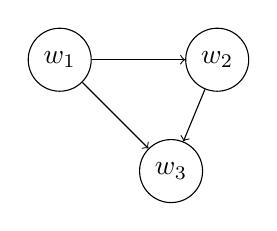
\begin{tikzpicture}[node distance=2cm, every node/.style={circle, draw, minimum size=0.8cm}]
    \node (w1) {$w_1$};
    \node (w2) [right of=w1] {$w_2$};
    \node (w3) [below right of=w1] {$w_3$};
    \draw[->] (w1) -- (w2);
    \draw[->] (w1) -- (w3);
    \draw[->] (w2) -- (w3);
\end{tikzpicture}
\end{center}

From $w_1$, both $w_2$ and $w_3$ are accessible. From $w_2$, only $w_3$ is accessible. From $w_3$, nothing is accessible.
\end{example}

To evaluate formulas, we need to know which propositions are true at which worlds:

\begin{definition}[Kripke Model]
A \emph{Kripke model} is a triple $\mathcal{M} = (W, R, V)$ where:
\begin{itemize}
    \item $(W, R)$ is a Kripke frame
    \item $V : \mathrm{Prop} \to \mathcal{P}(W)$ is a \emph{valuation}---for each proposition $p$, $V(p)$ is the set of worlds where $p$ is true
\end{itemize}
\end{definition}

\section{Satisfaction: When is a Formula True?}

Now the key question: given a model $\mathcal{M}$ and a world $w$, when is a formula $\varphi$ true?

We write $\mathcal{M}, w \models \varphi$ to mean ``$\varphi$ is true at world $w$ in model $\mathcal{M}$.''

\begin{definition}[Satisfaction Relation]
Let $\mathcal{M} = (W, R, V)$ and $w \in W$. We define $\models$ recursively:

\begin{center}
\begin{tabular}{lcp{7cm}}
$\mathcal{M}, w \models p$ & iff & $w \in V(p)$ \\
& & \textit{``$p$ is true at $w$''} \\[0.5em]
$\mathcal{M}, w \models \neg\varphi$ & iff & $\mathcal{M}, w \not\models \varphi$ \\
& & \textit{``$\varphi$ is not true at $w$''} \\[0.5em]
$\mathcal{M}, w \models \varphi \land \psi$ & iff & $\mathcal{M}, w \models \varphi$ and $\mathcal{M}, w \models \psi$ \\
& & \textit{``both are true at $w$''} \\[0.5em]
$\mathcal{M}, w \models \necessary\varphi$ & iff & for all $v$ with $wRv$: $\mathcal{M}, v \models \varphi$ \\
& & \textit{``$\varphi$ is true at ALL accessible worlds''} \\[0.5em]
$\mathcal{M}, w \models \possible\varphi$ & iff & there exists $v$ with $wRv$: $\mathcal{M}, v \models \varphi$ \\
& & \textit{``$\varphi$ is true at SOME accessible world''}
\end{tabular}
\end{center}
\end{definition}

\begin{intuition}
$\necessary$ means ``in all accessible worlds'' and $\possible$ means ``in some accessible world.''

If no worlds are accessible from $w$, then:
\begin{itemize}
    \item $\necessary\varphi$ is \textbf{vacuously true} (there's no accessible world where $\varphi$ could fail)
    \item $\possible\varphi$ is \textbf{false} (there's no accessible world where $\varphi$ could hold)
\end{itemize}
\end{intuition}

\begin{example}[Evaluating formulas]
Consider this model with $V(p) = \{w_1, w_3\}$ (meaning $p$ is true at $w_1$ and $w_3$):

\begin{center}
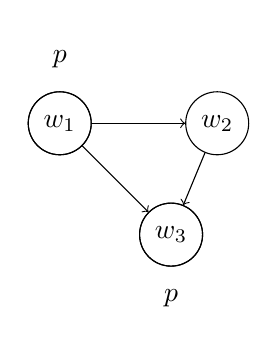
\begin{tikzpicture}[node distance=2cm, every node/.style={circle, draw, minimum size=0.8cm}]
    \node (w1) {$w_1$};
    \node[label=above:{$p$}] (w1l) at (w1) {};
    \node (w2) [right of=w1] {$w_2$};
    \node (w3) [below right of=w1] {$w_3$};
    \node[label=below:{$p$}] (w3l) at (w3) {};
    \draw[->] (w1) -- (w2);
    \draw[->] (w1) -- (w3);
    \draw[->] (w2) -- (w3);
\end{tikzpicture}
\end{center}

Let's evaluate some formulas at $w_1$:
\begin{itemize}
    \item $\mathcal{M}, w_1 \models p$? \textbf{Yes}, because $w_1 \in V(p)$.
    \item $\mathcal{M}, w_1 \models \necessary p$? \textbf{No}, because $w_2$ is accessible from $w_1$, but $p$ is false at $w_2$.
    \item $\mathcal{M}, w_1 \models \possible p$? \textbf{Yes}, because $w_3$ is accessible and $p$ is true there.
    \item $\mathcal{M}, w_2 \models \necessary p$? \textbf{Yes}, because the only world accessible from $w_2$ is $w_3$, and $p$ is true there.
\end{itemize}
\end{example}

\section{Frame Properties and Axioms}

Here's where it gets interesting: the \emph{properties of the accessibility relation} determine which formulas are valid.

Let's go through them one by one, with plain English first.

\subsection{Reflexivity and Axiom T}

\begin{quote}
\textbf{Property:} $R$ is reflexive---every world can access itself.

\textbf{Plain English meaning:} ``What is necessarily true is actually true.'' If something holds in ALL accessible worlds, and the current world is accessible from itself, then it holds here too.

\textbf{Axiom T:} $\necessary\varphi \to \varphi$

\textbf{Read as:} ``If $\varphi$ is necessarily true, then $\varphi$ is true.''
\end{quote}

\begin{intuition}
This axiom says you can't escape reality. If something is true in all possibilities, it's true in this one---because this one is a possibility.

Without reflexivity, you could have $\necessary\varphi$ true at $w$ (all accessible worlds satisfy $\varphi$) while $\varphi$ is false at $w$ itself (because $w$ doesn't access itself).
\end{intuition}

\subsection{Transitivity and Axiom 4}

\begin{quote}
\textbf{Property:} $R$ is transitive---if $w$ accesses $v$, and $v$ accesses $u$, then $w$ accesses $u$.

\textbf{Plain English meaning:} ``What is necessarily true is necessarily necessarily true.'' If $\varphi$ holds in all accessible worlds, then from any of those worlds, $\varphi$ still holds in all \emph{their} accessible worlds.

\textbf{Axiom 4:} $\necessary\varphi \to \necessary\necessary\varphi$

\textbf{Read as:} ``If $\varphi$ is necessarily true, then it's necessarily necessary.''
\end{quote}

\begin{intuition}
This is about \emph{positive introspection} in epistemic logic: if you know something, you know that you know it.

Without transitivity, you might know $\varphi$ (it's true in all worlds you consider possible), but from some of those worlds, there are further worlds you can't ``see'' from here---and $\varphi$ might fail there.
\end{intuition}

\subsection{Symmetry and Axiom B}

\begin{quote}
\textbf{Property:} $R$ is symmetric---if $w$ accesses $v$, then $v$ accesses $w$.

\textbf{Plain English meaning:} ``What is true is necessarily possible.'' If $\varphi$ is true here, then from any accessible world, this world is accessible back, so $\varphi$ is possible there.

\textbf{Axiom B:} $\varphi \to \necessary\possible\varphi$

\textbf{Read as:} ``If $\varphi$ is true, then necessarily $\varphi$ is possible.''
\end{quote}

\begin{intuition}
This says you can always ``get back.'' If from here, world $v$ looks possible, then from $v$, here looks possible too.
\end{intuition}

\subsection{Euclideanness and Axiom 5}

\begin{quote}
\textbf{Property:} $R$ is Euclidean---if $w$ accesses both $v$ and $u$, then $v$ accesses $u$.

\textbf{Plain English meaning:} ``What is possible is necessarily possible.'' If $\varphi$ is possible (true at some accessible world $v$), then from any accessible world $u$, you can still reach $v$.

\textbf{Axiom 5:} $\possible\varphi \to \necessary\possible\varphi$

\textbf{Read as:} ``If $\varphi$ is possible, then it's necessarily possible.''
\end{quote}

\begin{intuition}
This is about \emph{negative introspection}: if you don't know something (i.e., it's possible that not-$\varphi$), then you know that you don't know it.

With a Euclidean relation, all accessible worlds can see each other.
\end{intuition}

\subsection{Summary Table}

\begin{center}
\begin{tabular}{llll}
\textbf{Property} & \textbf{Axiom} & \textbf{Name} & \textbf{Plain reading} \\
\hline
Reflexive & $\necessary\varphi \to \varphi$ & T & ``Necessary implies true'' \\
Transitive & $\necessary\varphi \to \necessary\necessary\varphi$ & 4 & ``Necessary implies necessarily necessary'' \\
Symmetric & $\varphi \to \necessary\possible\varphi$ & B & ``True implies necessarily possible'' \\
Euclidean & $\possible\varphi \to \necessary\possible\varphi$ & 5 & ``Possible implies necessarily possible'' \\
\end{tabular}
\end{center}

\begin{history}
The names T, 4, B, 5 come from C.I. Lewis's systems S1--S5 of modal logic. S5, the strongest, assumes $R$ is an equivalence relation (reflexive + symmetric + transitive, or equivalently reflexive + Euclidean). In S5, the modal operators collapse: $\necessary\necessary\varphi \equiv \necessary\varphi$ and $\possible\necessary\varphi \equiv \necessary\varphi$.
\end{history}

\section{Bisimulation: The Right Notion of Equivalence}

When are two models ``the same'' from a modal logic perspective?

Not when they're literally identical---that's too strict. We want: \textbf{two models are equivalent if no modal formula can tell them apart.}

\begin{definition}[Bisimulation]
Let $\mathcal{M} = (W, R, V)$ and $\mathcal{M}' = (W', R', V')$ be Kripke models. A relation $Z \subseteq W \times W'$ is a \emph{bisimulation} if whenever $wZw'$:
\begin{enumerate}
    \item \textbf{(Atoms)} $w$ and $w'$ agree on all propositions: $w \in V(p) \Leftrightarrow w' \in V'(p)$ for all $p$
    \item \textbf{(Zig)} If $w$ can step to $v$ (i.e., $wRv$), then $w'$ can step to some $v'$ with $vZv'$
    \item \textbf{(Zag)} If $w'$ can step to $v'$ (i.e., $w'R'v'$), then $w$ can step to some $v$ with $vZv'$
\end{enumerate}
We write $w \bisim w'$ if there exists a bisimulation $Z$ with $wZw'$.
\end{definition}

\begin{intuition}
Bisimulation says: ``whatever move you make, I can match it.'' It's like a game:
\begin{itemize}
    \item If you step from $w$ to $v$, I can step from $w'$ to some $v'$ that's still bisimilar to $v$.
    \item And vice versa.
\end{itemize}
Neither player can ``escape'' to a state the other can't match.
\end{intuition}

\begin{theorem}[Bisimulation Invariance]
If $w \bisim w'$, then for all modal formulas $\varphi$:
\[
\mathcal{M}, w \models \varphi \iff \mathcal{M}', w' \models \varphi
\]
\end{theorem}

\begin{proofsketch}
By induction on $\varphi$:
\begin{itemize}
    \item Base case ($p$): By the Atoms condition, $w \in V(p) \Leftrightarrow w' \in V'(p)$.
    \item Boolean cases ($\neg$, $\land$): By induction hypothesis.
    \item Modal case ($\necessary\varphi$): If $\mathcal{M}, w \models \necessary\varphi$, then $\varphi$ holds at all successors of $w$. For any successor $v'$ of $w'$, by Zag there's a matching successor $v$ of $w$ with $vZv'$. By IH, $\varphi$ holds at $v'$. So $\mathcal{M}', w' \models \necessary\varphi$. Similarly for the other direction using Zig.
\end{itemize}
\end{proofsketch}

\begin{keyinsight}
Bisimulation is the ``right'' equivalence for modal logic:
\begin{itemize}
    \item Two bisimilar states satisfy exactly the same modal formulas.
    \item Conversely, over image-finite models, states satisfying the same formulas are bisimilar (Hennessy-Milner theorem).
\end{itemize}
This notion will generalize to \textbf{coalgebra}, where it becomes the universal notion of behavioral equivalence.
\end{keyinsight}

\begin{summary}
\begin{itemize}
    \item A \textbf{relation} on $W$ is a set of pairs $R \subseteq W \times W$
    \item Relations can be reflexive, symmetric, transitive (and combinations)
    \item An \textbf{equivalence relation} is all three
    \item A \textbf{Kripke frame} is a set of worlds + an accessibility relation
    \item A \textbf{Kripke model} adds a valuation saying which propositions are true where
    \item $\necessary\varphi$ means ``true at all accessible worlds''; $\possible\varphi$ means ``true at some''
    \item Frame properties (reflexive, transitive, ...) correspond to axioms (T, 4, ...)
    \item \textbf{Bisimulation} is the right notion of equivalence: bisimilar states satisfy the same modal formulas
\end{itemize}
\end{summary}
